%%%%%%%%%%%%%%%%%%%%%%%%%%%%%%%%%%%%%%%%%%%%%%%%%%%%%%%%%%%%%%%%%%%%
% Author: Juan Jose Herrera Aranda 
% Date: Agosto - 2022
% University of Granada
%%%%%%%%%%%%%%%%%%%%%%%%%%%%%%%%%%%%%%%%%%%%%%%%%%%%%%%%%%%%%%%%%%%%

\documentclass[11pt,a4paper, compress,graphics]{beamer}

\usepackage{slides}
\usepackage{tikz}
\usetikzlibrary{arrows.meta}
\usepackage{pgfplots}

%----------------------------------------------------------------------------------------
%	TITLE, AUTHOR AND OTHER INFO
%----------------------------------------------------------------------------------------


% Title of the document.
\newcommand{\doctitle}{Desarrollo de modelos de Deep Learning basados en redes neuronales recurrentes para clasificación de electrocardiogramas}
% Subtitle.
\newcommand{\docsubtitle}{Trabajo Fin de Grado}
% Date.
\newcommand{\docdate}{Septiembre 2022}
% Author.
\newcommand{\docauthor}{Juan José Herrera Aranda}
\newcommand{\docaddress}{Universidad de Granada}
\newcommand{\docemail}{jh16357@gmail.com}

\title{\doctitle}
\author{\docauthor}


%-----------------------------------------------------------------------------------------------------
%	TITLE PAGE
%-----------------------------------------------------------------------------------------------------
%en corchetes ponemos nombres más cortos, para mejor visualización de las cabeceras del documento

%\title[Taller de \LaTeX]{Taller de \LaTeX\ yosigopublicando}
%\author[Los presentes]{Juan José Herrera Aranda}
%\institute[UGR]{Universidad de Granada}

\titlegraphic{

\includegraphics[width=2cm,height=2cm]{Images/UGR.jpg}
}

\begin{document}
	


%----------------------------------------------------------------------------------------
%	Title page.
%----------------------------------------------------------------------------------------

{
%	\usebackgroundtemplate{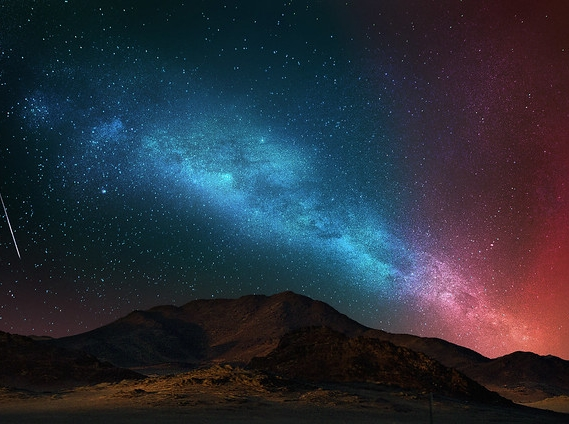
\includegraphics[width=1\paperwidth]{./Images/background.jpg}}
	\begin{frame}
        \titlepage 
	\end{frame}
}

\section*{Índice}
% Table of contents
\begin{frame}
	\tableofcontents[hideallsubsections]
\end{frame}

%----------------------------------------------------------------------------------------
%	Motivation
%----------------------------------------------------------------------------------------
\importsection{motivation}


%****************************************************************************************
%*************************         MATEMÁTICAS       ************************************
%****************************************************************************************

%----------------------------------------------------------------------------------------
%	Teoría del Aprendizaje Estadístico
%----------------------------------------------------------------------------------------
\importsection{AprendizajeEstadistico}

%----------------------------------------------------------------------------------------
%	Teorema de Aproximación Universal
%----------------------------------------------------------------------------------------
\importsection{TeoremaAU}



%****************************************************************************************
%*************************         INFORMÁTICA       ************************************
%****************************************************************************************

%----------------------------------------------------------------------------------------
%	Motivation
%----------------------------------------------------------------------------------------
\importsection{RedesNeuronales}


%****************************************************************************************
%***************************         CLASIFICACIÓN       ********************************
%****************************************************************************************

%----------------------------------------------------------------------------------------
%	Descripción del problema
%----------------------------------------------------------------------------------------
\importsection{descripcion_problema}

%----------------------------------------------------------------------------------------
%	Resultados Analisis
%----------------------------------------------------------------------------------------
\importsection{ResultadosAnalisis}

%----------------------------------------------------------------------------------------
%	Conclusion
%----------------------------------------------------------------------------------------

\importsection{conclusion}


%----------------------------------------------------------------------------------------
%	Last slide
%----------------------------------------------------------------------------------------

\section*{Fin}

\begin{frame}
\begin{center}
    \vspace{1cm}
    {\Large \textbf{\textit{Muchas gracias por la atención}}}
\end{center}  

    \begin{center}
        \vspace{2cm}
        {\Large \textbf{\textit{Hasta la próxima :)}}}
    \end{center}
\end{frame}


\end{document}